\documentclass{amsart}

% Notes:
% 1. too many tikz options may cause errors
% 2. install https://github.com/michal-h21/dvisvgm4ht
%   - add the following

\ifdefined\HCode
  \def\pgfsysdriver{pgfsys-tex4ht-updated.def}
\fi 

% 3. run `'$ make4ht -f html5+dvisvgm_hashes tikz-test.tex  "mathjax"`'
% 4. SVG files may be populated with (invalid) stray closing </p> tags
%   - manual fix

\usepackage{tikz}\usetikzlibrary{positioning}

\begin{document}

hello, world

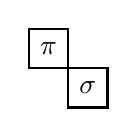
\begin{tikzpicture}[scale=0.5, baseline=(current bounding box.center)]
  \draw[thick, line cap=round] (0,1) rectangle (1,2);
  \draw[thick, line cap=round] (1,0) rectangle (2,1);
  \node at (0.5,1.5) {$\pi$};
  \node at (1.5,0.5) {$\sigma$};
\end{tikzpicture}

\begin{tikzpicture}\draw (-2,0) -- (2,0);    \filldraw [gray] (0,0) circle (2pt);\draw (-2,-2) .. controls (0,0) .. (2,-2);    \draw (-2,2) .. controls (-1,0) and (1,0) .. (2,2);\end{tikzpicture}

\begin{equation} \label{tikzPic}
    x = \begin{tikzpicture}
    \draw (-2,0) -- (2,0);
    \draw[fill=gray] (0,0) circle (2pt);
    \draw (-2,-2) .. controls (0,0) .. (2,-2);
    \draw (-2,2) .. controls (-1,0) and (1,0) .. (2,2);
    \end{tikzpicture}
\end{equation}

And standalone

\Picture*[alt text]{fallback-filename}
some text  as image
\EndPicture


\end{document}
